\documentclass[tikz,border=5pt]{standalone}
\usepackage{times}
\usepackage[T1]{fontenc}
\usepackage[utf8]{inputenc}
\usepackage{amsmath,amssymb}
\usepackage{xcolor}
\usetikzlibrary{arrows.meta,positioning,calc,fit,backgrounds,shapes.geometric}

% Palette matching ACL/ICLR figures
\definecolor{residpurple}{HTML}{EDE9FE}
\definecolor{residborder}{HTML}{7C3AED}
\definecolor{attnblue}{HTML}{DBEAFE}
\definecolor{attnborder}{HTML}{2563EB}
\definecolor{mlpteal}{HTML}{CCFBF1}
\definecolor{mlpborder}{HTML}{0D9488}
\definecolor{unembyellow}{HTML}{FEF3C7}
\definecolor{unembborder}{HTML}{D97706}
\definecolor{medgreen}{HTML}{059669}
\definecolor{medbg}{HTML}{ECFDF5}
\definecolor{bypred}{HTML}{DC2626}
\definecolor{bypbg}{HTML}{FEF2F2}
\definecolor{cleanamber}{HTML}{FCD34D}
\definecolor{cleanborder}{HTML}{D97706}
\definecolor{editpink}{HTML}{F472B6}
\definecolor{editborder}{HTML}{BE185D}
\definecolor{faintpink}{HTML}{FCE7F3}
\definecolor{slate}{HTML}{334155}

\begin{document}
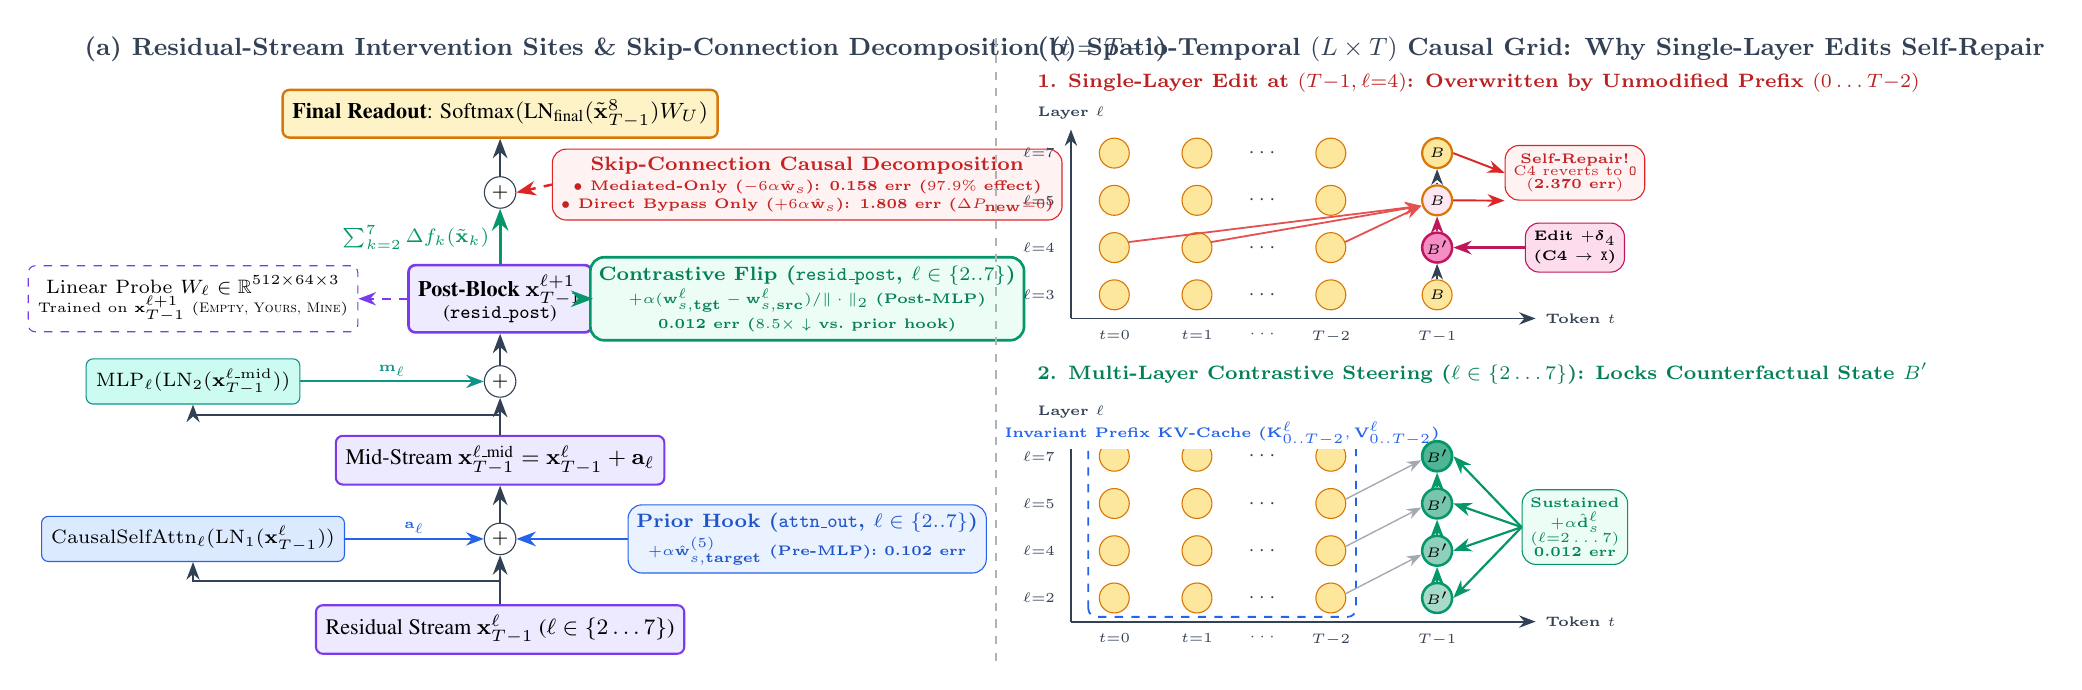
\begin{tikzpicture}[
    font=\fontfamily{ptm}\selectfont\footnotesize,
    >=Stealth,
    box/.style={draw, rounded corners=2.5pt, align=center, minimum height=0.52cm, inner sep=3.5pt},
    residnode/.style={box, fill=residpurple, draw=residborder, line width=0.75pt, minimum width=2.55cm},
    subnode/.style={box, minimum width=2.25cm, minimum height=0.46cm, font=\scriptsize},
    pill/.style={draw, rounded corners=5pt, inner sep=3pt, font=\scriptsize\bfseries, align=center},
    toknode/.style={circle, draw, minimum size=0.38cm, inner sep=0pt, font=\tiny\bfseries}
]

% =========================================================================
% PANEL (a): RESIDUAL STREAM & CAUSAL DECOMPOSITION AT TIMESTEP T-1
% =========================================================================
\node[anchor=north west, font=\small\bfseries, text=slate] at (-1.85, 7.85)
    {(a) Residual-Stream Intervention Sites \& Skip-Connection Decomposition ($t = T{-}1$)};

% Bottom input
\node[residnode] (x2) at (3.55, 0.2) {Residual Stream $\mathbf{x}_{T-1}^{\ell}$ ($\ell \in \{2\dots 7\}$)};

% Attention subblock
\node[subnode, fill=attnblue, draw=attnborder] (attn) at (-0.35, 1.35)
    {$\text{CausalSelfAttn}_\ell(\text{LN}_1(\mathbf{x}_{T-1}^\ell))$};
\node[circle, draw=slate, fill=white, inner sep=1.2pt, font=\scriptsize\bfseries] (add1) at (3.55, 1.35) {$+$};

% Mid residual
\node[residnode] (xmid) at (3.55, 2.35) {Mid-Stream $\mathbf{x}_{T-1}^{\ell\text{\_mid}} = \mathbf{x}_{T-1}^\ell + \mathbf{a}_\ell$};

% MLP subblock
\node[subnode, fill=mlpteal, draw=mlpborder] (mlp) at (-0.35, 3.35)
    {$\text{MLP}_\ell(\text{LN}_2(\mathbf{x}_{T-1}^{\ell\text{\_mid}}))$};
\node[circle, draw=slate, fill=white, inner sep=1.2pt, font=\scriptsize\bfseries] (add2) at (3.55, 3.35) {$+$};

% Post residual (where probes W_l are trained!)
\node[residnode, fill=residpurple!90!white, line width=0.95pt, minimum width=2.2cm] (xpost) at (3.55, 4.40)
    {\textbf{Post-Block} $\mathbf{x}_{T-1}^{\ell+1}$\\[-1.5pt]{\scriptsize (\texttt{resid\_post})}};

% Probe readout callout on the left of xpost
\node[box, fill=white, draw=residborder, dashed, font=\scriptsize, minimum width=2.30cm] (probe) at (-0.35, 4.40)
    {Linear Probe $W_\ell \in \mathbb{R}^{512 \times 64 \times 3}$\\[-1pt]
    {\tiny Trained on $\mathbf{x}_{T-1}^{\ell+1}$ (\textsc{Empty, Yours, Mine})}};
\draw[->, dashed, residborder, line width=0.75pt] (xpost.west) -- (probe.east);

% Final layer norm & Unembed
\node[circle, draw=slate, fill=white, inner sep=1.2pt, font=\scriptsize\bfseries] (addfinal) at (3.55, 5.75) {$+$};
\node[box, fill=unembyellow, draw=unembborder, line width=0.85pt, minimum width=3.1cm, minimum height=0.58cm] (unemb) at (3.55, 6.75)
    {\textbf{Final Readout}: $\text{Softmax}(\text{LN}_{\text{final}}(\tilde{\mathbf{x}}_{T-1}^8) W_U)$};

% Backbone arrows
\draw[->, line width=0.9pt, slate] (x2.north) -- (add1.south);
\draw[->, line width=0.75pt, slate] (x2.north) -- ++(0, 0.30) -| (attn.south);
\draw[->, line width=0.75pt, attnborder] (attn.east) -- node[above, font=\tiny, inner sep=1.5pt]{$\mathbf{a}_\ell$} (add1.west);
\draw[->, line width=0.9pt, slate] (add1.north) -- (xmid.south);

\draw[->, line width=0.9pt, slate] (xmid.north) -- (add2.south);
\draw[->, line width=0.75pt, slate] (xmid.north) -- ++(0, 0.25) -| (mlp.south);
\draw[->, line width=0.75pt, mlpborder] (mlp.east) -- node[above, font=\tiny, inner sep=1.5pt]{$\mathbf{m}_\ell$} (add2.west);
\draw[->, line width=0.9pt, slate] (add2.north) -- (xpost.south);

\draw[->, line width=1.1pt, medgreen] (xpost.north) -- node[left, font=\scriptsize\bfseries, text=medgreen, pos=0.48]
    {$\sum_{k=2}^7 \Delta f_k(\tilde{\mathbf{x}}_k)$} (addfinal.south);
\draw[->, line width=0.9pt, slate] (addfinal.north) -- (unemb.south);

% Right-side Intervention Callouts (3 distinct pathways tested)
% 1. Site A: Nanda et al. attn_out hook
\node[pill, fill=attnblue!60, draw=attnborder, text=attnborder!85!black, minimum width=3.55cm] (nanda_hook) at (7.45, 1.35)
    {\textbf{Prior Hook} (\texttt{attn\_out}, $\ell \in \{2..7\}$)\\[0.5pt]
    {\tiny $+\alpha \hat{\mathbf{w}}_{s,\text{target}}^{(5)}$ (Pre-MLP): \textbf{0.102 err}}};
\draw[->, line width=0.9pt, attnborder] (nanda_hook.west) -- (add1.east);

% 2. Site B: Our Contrastive Flip @ resid_post
\node[pill, fill=medbg, draw=medgreen, text=medgreen!85!black, line width=0.95pt, minimum width=3.55cm] (our_hook) at (7.45, 4.40)
    {\textbf{Contrastive Flip} (\texttt{resid\_post}, $\ell \in \{2..7\}$)\\[0.5pt]
    {\tiny $+\alpha (\mathbf{w}_{s,\text{tgt}}^\ell - \mathbf{w}_{s,\text{src}}^\ell) / \|\cdot\|_2$ (Post-MLP)}\\[1pt]
    {\tiny \textbf{0.012 err ($8.5\times \downarrow$ vs.\ prior hook)}}};
\draw[->, line width=1.1pt, medgreen] (our_hook.west) -- (xpost.east);

% 3. Skip-connection decomposition at addfinal
\node[pill, fill=bypbg, draw=bypred, text=bypred!90!black, minimum width=3.55cm] (skip_hook) at (7.45, 5.85)
    {\textbf{Skip-Connection Causal Decomposition}\\[-1pt]
    {\tiny $\bullet$ \textbf{Mediated-Only} ($-6\alpha\hat{\mathbf{w}}_s$): \textbf{0.158 err} ($97.9\%$ effect)}\\[-1.5pt]
    {\tiny $\bullet$ \textbf{Direct Bypass Only} ($+6\alpha\hat{\mathbf{w}}_s$): \textbf{1.808 err} ($\Delta P_{\text{new}}{=}0$)}};
\draw[->, line width=0.9pt, bypred, dashed] (skip_hook.west) -- (addfinal.east);

% Subtle divider line between Panel (a) and Panel (b)
\draw[slate!40, line width=0.7pt, dashed] (9.85, -0.2) -- (9.85, 7.8);

% =========================================================================
% PANEL (b): SPATIO-TEMPORAL (L x T) CAUSAL GRID & SELF-REPAIR
% =========================================================================
\node[anchor=north west, font=\small\bfseries, text=slate] at (10.25, 7.85)
    {(b) Spatio-Temporal $(L \times T)$ Causal Grid: Why Single-Layer Edits Self-Repair};

% --- SUBGRID 1: SINGLE-LAYER EDIT AT L4 (TOP RIGHT) ---
\node[anchor=west, font=\scriptsize\bfseries, text=bypred!85!black] at (10.25, 7.15)
    {1. Single-Layer Edit at $(T{-}1, \ell{=}4)$: Overwritten by Unmodified Prefix $(0\dots T{-}2)$};

% Draw axes for Subgrid 1
\draw[->, slate, line width=0.65pt] (10.8, 4.15) -- (10.8, 6.55) node[above, font=\tiny\bfseries]{Layer $\ell$};
\draw[->, slate, line width=0.65pt] (10.8, 4.15) -- (16.7, 4.15) node[right, font=\tiny\bfseries]{Token $t$};

\foreach \y/\ly in {4.45/\ell{=}3, 5.05/\ell{=}4, 5.65/\ell{=}5, 6.25/\ell{=}7} {
    \node[font=\tiny, anchor=east, text=slate] at (10.72, \y) {$\ly$};
}
\foreach \x/\tx in {11.35/t{=}0, 12.40/t{=}1, 13.25/\cdots, 14.10/T{-}2, 15.45/T{-}1} {
    \node[font=\tiny, anchor=north, text=slate] at (\x, 4.12) {$\tx$};
}

% Prefix tokens (unmodified amber)
\foreach \y in {4.45, 5.05, 5.65, 6.25} {
    \node[toknode, fill=cleanamber!55, draw=cleanborder] at (11.35, \y) {};
    \node[toknode, fill=cleanamber!55, draw=cleanborder] at (12.40, \y) {};
    \node[font=\scriptsize, text=slate] at (13.25, \y) {$\cdots$};
    \node[toknode, fill=cleanamber!55, draw=cleanborder] at (14.10, \y) {};
}

% T-1 column in Subgrid 1
\node[toknode, fill=cleanamber!55, draw=cleanborder] (s1_t3) at (15.45, 4.45) {$B$};
\node[toknode, fill=editpink!80, draw=editborder, line width=0.9pt] (s1_t4) at (15.45, 5.05) {$B'$};
\node[toknode, fill=faintpink, draw=cleanborder, line width=0.8pt] (s1_t5) at (15.45, 5.65) {$B$};
\node[toknode, fill=cleanamber!55, draw=cleanborder, line width=0.8pt] (s1_t7) at (15.45, 6.25) {$B$};

\draw[->, slate, line width=0.6pt] (s1_t3) -- (s1_t4);
\draw[->, editborder, line width=0.7pt] (s1_t4) -- (s1_t5);
\draw[->, slate, line width=0.6pt, dotted] (s1_t5) -- (s1_t7);

% Causal attention washout arrows from prefix at l=4 into (T-1, l=5)
\draw[->, bypred!80, line width=0.65pt] (11.53, 5.12) -- (15.25, 5.58);
\draw[->, bypred!80, line width=0.65pt] (12.58, 5.12) -- (15.25, 5.58);
\draw[->, bypred!80, line width=0.65pt] (14.28, 5.12) -- (15.25, 5.58);

% Callout on Subgrid 1
\node[pill, fill=editpink!25, draw=editborder, font=\tiny\bfseries] (inj1) at (17.20, 5.05)
    {Edit $+\boldsymbol{\delta}_4$\\[1pt](C4 $\to$ \texttt{X})};
\draw[->, editborder, line width=0.8pt] (inj1.west) -- (s1_t4.east);

\node[pill, fill=bypbg, draw=bypred, font=\tiny, text=bypred!90!black] (rep1) at (17.20, 6.00)
    {\textbf{Self-Repair!}\\[-1.5pt]C4 reverts to \texttt{O}\\[-1.5pt](\textbf{2.370 err})};
\draw[->, bypred, line width=0.7pt] (s1_t5.east) -- (rep1.south west);
\draw[->, bypred, line width=0.7pt] (s1_t7.east) -- (rep1.west);

% --- SUBGRID 2: SUSTAINED MULTI-LAYER STEERING L2..7 (BOTTOM RIGHT) ---
\node[anchor=west, font=\scriptsize\bfseries, text=medgreen!85!black] at (10.25, 3.45)
    {2. Multi-Layer Contrastive Steering ($\ell \in \{2\dots 7\}$): Locks Counterfactual State $B'$};

% Draw axes for Subgrid 2
\draw[->, slate, line width=0.65pt] (10.8, 0.30) -- (10.8, 2.75) node[above, font=\tiny\bfseries]{Layer $\ell$};
\draw[->, slate, line width=0.65pt] (10.8, 0.30) -- (16.7, 0.30) node[right, font=\tiny\bfseries]{Token $t$};

\foreach \y/\ly in {0.60/\ell{=}2, 1.20/\ell{=}4, 1.80/\ell{=}5, 2.40/\ell{=}7} {
    \node[font=\tiny, anchor=east, text=slate] at (10.72, \y) {$\ly$};
}
\foreach \x/\tx in {11.35/t{=}0, 12.40/t{=}1, 13.25/\cdots, 14.10/T{-}2, 15.45/T{-}1} {
    \node[font=\tiny, anchor=north, text=slate] at (\x, 0.27) {$\tx$};
}

% Prefix tokens (unmodified amber, KV-cached!)
\foreach \y in {0.60, 1.20, 1.80, 2.40} {
    \node[toknode, fill=cleanamber!55, draw=cleanborder] at (11.35, \y) {};
    \node[toknode, fill=cleanamber!55, draw=cleanborder] at (12.40, \y) {};
    \node[font=\scriptsize, text=slate] at (13.25, \y) {$\cdots$};
    \node[toknode, fill=cleanamber!55, draw=cleanborder] at (14.10, \y) {};
}

% Highlight KV-cache box around prefix tokens
\draw[attnborder, dashed, rounded corners=3pt, line width=0.65pt] (11.02, 0.36) rectangle (14.42, 2.68);
\node[font=\tiny\bfseries, text=attnborder, fill=white, inner sep=1pt] at (12.72, 2.68)
    {Invariant Prefix KV-Cache ($\mathbf{K}_{0..T-2}^\ell, \mathbf{V}_{0..T-2}^\ell$)};

% T-1 column in Subgrid 2 (All locked to B'!)
\node[toknode, fill=medgreen!35, draw=medgreen, line width=0.9pt] (s2_t2) at (15.45, 0.60) {$B'$};
\node[toknode, fill=medgreen!45, draw=medgreen, line width=0.9pt] (s2_t4) at (15.45, 1.20) {$B'$};
\node[toknode, fill=medgreen!55, draw=medgreen, line width=0.9pt] (s2_t5) at (15.45, 1.80) {$B'$};
\node[toknode, fill=medgreen!70, draw=medgreen, line width=1.0pt] (s2_t7) at (15.45, 2.40) {$B'$};

\draw[->, medgreen, line width=0.8pt] (s2_t2) -- (s2_t4);
\draw[->, medgreen, line width=0.8pt] (s2_t4) -- (s2_t5);
\draw[->, medgreen, line width=0.8pt] (s2_t5) -- (s2_t7);

% Attention arrows from prefix
\foreach \yb/\yt in {0.60/1.20, 1.20/1.80, 1.80/2.40} {
    \draw[->, slate!45, line width=0.5pt] (14.28, \yb+0.05) -- (15.25, \yt-0.05);
}

% Multi-layer injection bracket on right
\node[pill, fill=medbg, draw=medgreen, font=\tiny\bfseries, text=medgreen!90!black] (inj2) at (17.20, 1.50)
    {Sustained\\[1pt]$+\alpha\hat{\mathbf{d}}_s^\ell$\\[-0.5pt]$(\ell{=}2\dots 7)$\\[-1pt]\textbf{0.012 err}};
\draw[->, medgreen, line width=0.8pt] (inj2.west) -- (s2_t2.east);
\draw[->, medgreen, line width=0.8pt] (inj2.west) -- (s2_t4.east);
\draw[->, medgreen, line width=0.8pt] (inj2.west) -- (s2_t5.east);
\draw[->, medgreen, line width=0.8pt] (inj2.west) -- (s2_t7.east);

\end{tikzpicture}
\end{document}
